\documentclass{article}
\usepackage[margin=1in, paperwidth=8.5in, paperheight=11in]{geometry}
\usepackage{caption}
\usepackage{subcaption}
\usepackage{float}
\usepackage{graphicx}
\usepackage[utf8]{inputenc}
\usepackage{hyperref}

\begin{document}


\subsection{Ready-To-Drive-Sound (RTDS)}
\subsubsection{Description}
%Describe your concept of the RTDS, how is the sound produced, what are the parameters for activating the RTDS, etc.
The Ready to Drive sound is located as a component of the dashboard subsystem, and contains a buzzer (\href{http://www.mallory-sonalert.com/specifications/STA20502.PDF}{Link: Mallory Sonalert Products Inc. STA20502})\ref{Ready to Drive}. The buzzer automatically makes a noise when given power, with the loudness proportional
to the voltage. The BMS will notify the Dashboard CAN system when shutdown circuit is complete. This will then provide voltage to the gate of an N-FET which will provide a ground path for the buzzer.
\subsubsection{Wiring, cables, current calculations, connectors}
%Describe wiring, show schematics, describe connectors and cables and show useful data regarding the wiring.
When the shutdown circuit closes and activates the AIRs, the car is in ready to drive mode. As soon as the
car is in this mode, the CAN system will activate the ready to drive sound node to send a positive output
that provides voltage to the N-FET for 2 seconds, thus letting the buzzer sound for 2 seconds. 


\begin{figure}[h]
	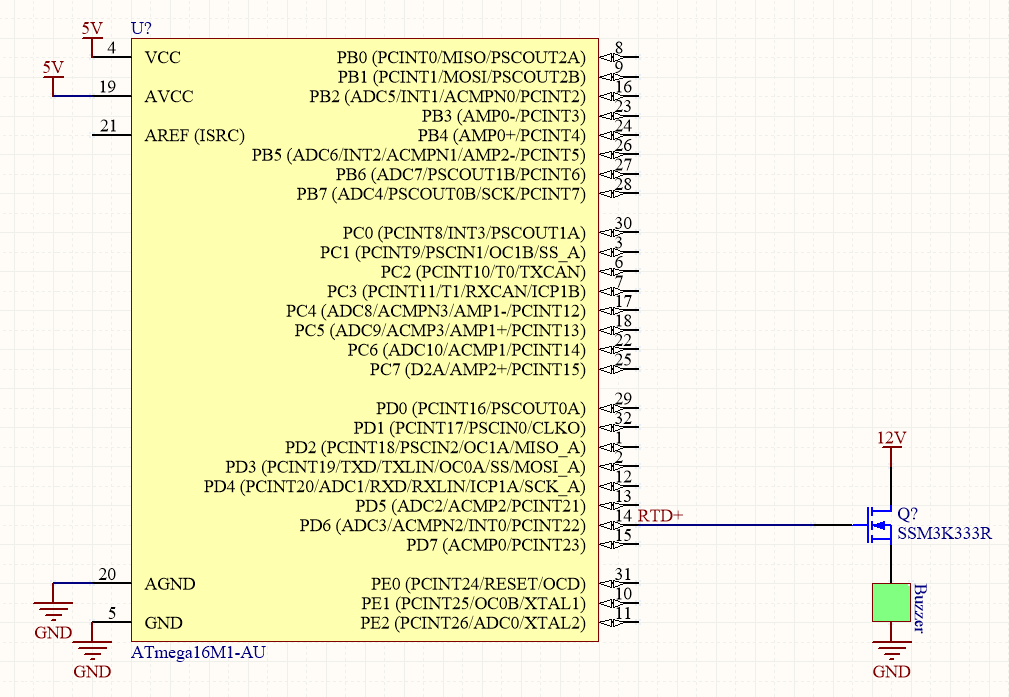
\includegraphics[width=\linewidth]{RTDS_Schematic_Simplified}
	\caption{Ready to Drive Sound Schematic as a subsystem of the dashboard's PCB}
\end{figure}
\begin{figure}[H]
	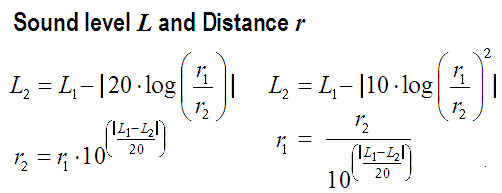
\includegraphics[width=\linewidth]{FormulasForDistanceAndSoundLevel}
	\caption{Inverse Square Law equations needed to calculate the volume at a certain distance}
\end{figure}
Using the inverse square law as referenced in the appendix  for sound pressure levels \ref{Ready to Drive}, 97db at 122cm will translate to 93db at 2m which is a loud enough volume without inducing harm to the listener. 
\subsubsection{Position in car}
%Provide CAD-renderings showing all relevant parts. Mark the parts in the rendering, if necessary.
The ready to drive sound will be located in the dashboard enclosure shown in Figure !!!!. The buzzer will be mounted
to the exterior and front side of this enclosure. It must be contained outside of the box so that the buzzer is
loud enough. The speaker is waterproof, so it doesn't require any extra protection besides using an RTV silicone seal for final instillation. 


\newpage
\subsection{Ready to Drive (APPENDIX SECTION)}\label{Ready to Drive}
Ready to drive buzzer \href{http://www.mallory-sonalert.com/specifications/STA20502.PDF}{datasheet}. \newline
\begin{figure}[H]
	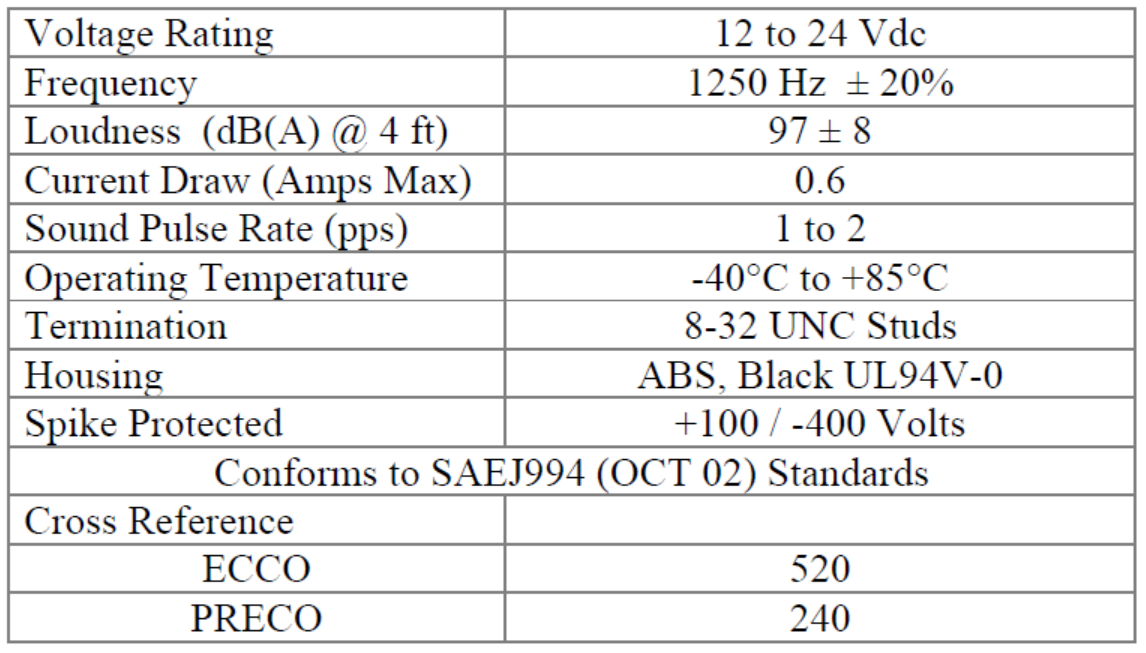
\includegraphics[width=\linewidth]{Buzzer_Specifications}
	\caption{Specification for Mallory Sonalert STA20502 Buzzer}
\end{figure}
For calculation of sound attenuation over distance, see \href{http://www.sengpielaudio.com/calculator-distance.htm}{SengpielAudio Distance Law Equation}
\end{document}
